\documentclass[a4paper]{arrowhead}

\usepackage[yyyymmdd]{datetime}
\usepackage{etoolbox}
\usepackage[utf8]{inputenc}
\usepackage{multirow}
\usepackage{hyperref}

\renewcommand{\dateseparator}{-}

\setlength{\parskip}{1em}

%% Special references
\newcommand{\fref}[1]{{\textcolor{ArrowheadBlue}{\hyperref[sec:functions:#1]{#1}}}}
\newcommand{\mref}[1]{{\textcolor{ArrowheadPurple}{\hyperref[sec:model:#1]{#1}}}}
\newcommand{\pdef}[1]{{\textcolor{ArrowheadGrey}{#1\label{sec:model:primitives:#1}\label{sec:model:primitives:#1s}\label{sec:model:primitives:#1es}}}}
\newcommand{\pref}[1]{{\textcolor{ArrowheadGrey}{\hyperref[sec:model:primitives:#1]{#1}}}}

\newrobustcmd\fsubsection[3]{
  \addtocounter{subsection}{1}
  \addcontentsline{toc}{subsection}{\protect\numberline{\thesubsection}function \textcolor{ArrowheadBlue}{#1}}
  \renewcommand*{\do}[1]{\rref{##1},\ }
  \subsection*{
    \thesubsection\quad
    operation
    \textcolor{ArrowheadBlue}{#1}
    (\notblank{#2}{\mref{#2}}{})
    \notblank{#3}{: \mref{#3}}{}
  }
  \label{sec:functions:#1}
}
\newrobustcmd\msubsection[2]{
  \addtocounter{subsection}{1}
  \addcontentsline{toc}{subsection}{\protect\numberline{\thesubsection}#1 \textcolor{ArrowheadPurple}{#2}}
  \subsection*{\thesubsection\quad#1 \textcolor{ArrowheadPurple}{#2}}
  \label{sec:model:#2} \label{sec:model:#2s} \label{sec:model:#2es}
}

\begin{document}

%% Arrowhead Document Properties
\ArrowheadTitle{Authorization Core System}
\ArrowheadType{System Description}
\ArrowheadTypeShort{SysD}
\ArrowheadVersion{4.6.0}
\ArrowheadDate{\today}
\ArrowheadAuthor{Tamás Bordi}
\ArrowheadStatus{RELEASE}
\ArrowheadContact{tbordi@aitia.ai}
\ArrowheadFooter{\href{www.arrowhead.eu}{www.arrowhead.eu}}
\ArrowheadSetup
%%

%% Front Page
\begin{center}
  \vspace*{1cm}
  \huge{\arrowtitle}

  \vspace*{0.2cm}
  \LARGE{\arrowtype}
  \vspace*{1cm}

  %\Large{Service ID: \textit{"\arrowid"}}
  \vspace*{\fill}

  % Front Page Image
  %\includegraphics{figures/TODO}

  \vspace*{1cm}
  \vspace*{\fill}

  % Front Page Abstract
  \begin{abstract}
    This document provides system description for the \textbf{Authorization Core System}.
  \end{abstract}

  \vspace*{1cm}

%   \scriptsize
%   \begin{tabularx}{\textwidth}{l X}
%     \raisebox{-0.5\height}{
\includegraphics[width=2cm]{figures/artemis_logo}} & {ARTEMIS Innovation Pilot Project: Arrowhead\newline
%     THEME [SP1-JTI-ARTEMIS-2012-AIPP4 SP1-JTI-ARTEMIS-2012-AIPP6]\newline
%     [Production and Energy System Automation Intelligent-Built environment and urban infrastructure for sustainable and friendly cities]}
%   \end{tabularx}
%   \vspace*{-0.2cm}
 \end{center}

\newpage
%%

%% Table of Contents
\tableofcontents
\newpage
%%

\section{Overview}
\label{sec:overview}
\color{black}
This document describes the Authorization Core System, which exists to manage and to authorize
connection between various systems using Authorization Rules within an Eclipse Arrowhead Local Cloud (LC). 

The rest of this document is organized as follows.
In Section \ref{sec:prior_art}, we reference major prior art capabilities
of the system.
In Section \ref{sec:use}, we describe the intended usage of the system.
In Section \ref{sec:properties}, we describe fundamental properties
provided by the system.
In Section \ref{sec:delimitations}, we describe delimitations of capabilities
of the system.
In Section \ref{sec:services}, we describe the abstract service
operations produced by the system.
In Section \ref{sec:security}, we describe the security capabilities
of the system.

\subsection{Significant Prior Art}
\label{sec:prior_art}

The strong development on cloud technology and various requirements for digitisation and automation has led to the concept of Local Clouds (LC).

\textit{"The concept takes the view that specific geographically local automation tasks should be encapsulated and protected."} \cite{jerker2017localclouds}

One of the main building blocks when realizing such Local Cloud is the capability of authorization and session control within the given LC.

\subsection{How This System Is Meant to Be Used}
\label{sec:use}

Authorization is a mandatory core system of Eclipse Arrowhead LC and is responsible for the fundamental authorization control functionality by storing applicable authorization rules. An intracloud rule describes an access policy between a consumer system and a provider system for a given service, interface pair, while an intercloud rule describes an access policy between a provider system and a neighbor cloud.

This core system is also responsible for providing the session control functionality which is achieved by providing a token generation service. 

\begin{figure}[h!]
  \centering
  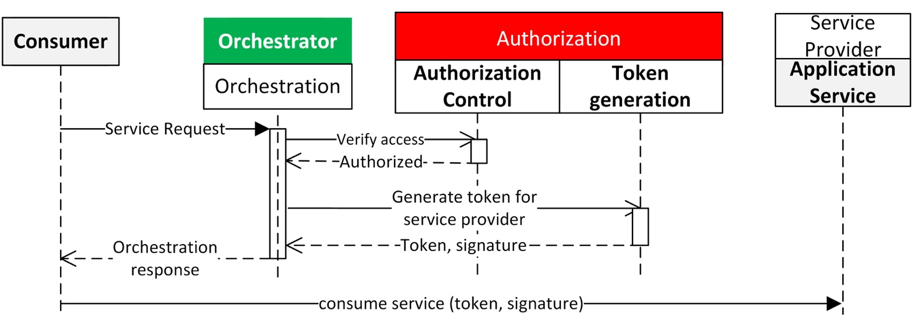
\includegraphics[width=15cm]{figures/authorization_control.png}
  \caption{
   Authorization crosscheck during orchestration process
  }
  \label{fig:information_overview}
\end{figure}

\subsection{System functionalities and properties}
\label{sec:properties}

\subsubsection {Functional properties of the system}
Authorization solves the following needs to fulfill the requirements of authorization and session control.

\begin{itemize}
    \item Enables the system operators to manually create and remove authorization rules.
    \item Enables the Orchestrator Core system to query the authorization rules during the orchestration process.
    \item Enables the Event Handler Core system to query the authorization rules during the subscription process.
    \item Enables the Orchestrator Core system to generate access tokens to the orchestrated provider, service and interface, when it is required.
    \item Enables the Choreographer Core system to re-generate tokens for executor systems.
    \item Enables the provider systems to get its public key in order to validate the token received from a consumer.
\end{itemize}

\subsubsection {Non functional properties of the system}
Beside the requirements of authorization and session control the Authorization Core System implements certain authentication of systems, meaning that the Authorization makes decision whether a given system has right to use its services or not.

\subsubsection {Data stored by the system}
In order to achieve the mentioned functionalities, Authorization is capable to store the information set described by figure \ref{fig:information_overview}.

\begin{figure}[h!]
  \centering
  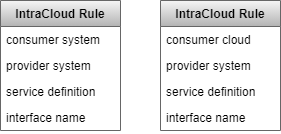
\includegraphics[width=8cm]{figures/authorization_data_overview.png}
  \caption{
    Overview of data stored by Authorization Core System.
  }
  \label{fig:information_overview}
\end{figure}

\subsection{Important Delimitations}
\label{sec:delimitations}

While Authorization Core System is responsible for applying the authorization rules, the rules itself can't be generated from higher level policies. System operators always have to define them on system, service definition and interface (database) record level. 

Also, the Authorization Core System can't operate without a running Service Registry Core System instances and the access token generation is only possible when the system is running in secure mode.

\newpage

\section{Services produced}
\label{sec:services}

\msubsection{service}{echo}
The purpose of this service is to test the system availability. The service is offered for both application and core systems. 

\msubsection{service}{authorization-control-intra}
The purpose of this service is to query for existing authorization rules for a specified consumer to a specified service definition with possible providers and interfaces. The service is offered only for specified core systems.

\msubsection{service}{authorization-control-inter}
The purpose of this service is to query for existing authorization rules for a specified consumer cloud to a specified service definition with possible providers and interfaces. The service is offered only for specified core systems.

\msubsection{service}{authorization-control-subscription}
The purpose of this service is to query for at least one existing authorization rule for a specified consumer to the specified providers. The service is offered only for specified core systems.

\msubsection{service}{token-generation}
The purpose of this service is to generate access tokens for a consumer to a provider with the content of service consumption session related data. The service is offered only for specified core systems.

\msubsection{service}{token-generation-multi-service}
The purpose of this service is to execute the \textit{token-generation} service, but for multiple consumers at once. The service is offered only for specified core systems.

\msubsection{service}{auth-public-key}
The purpose of this service is to provide the public key of the Authorization Core System. It is necessary for validating an access token generated by the Authorization. The service is offered for both application and core systems. 

\newpage

\section{Security}
\label{sec:security}

The security of Eclipse Arrowhead - and therefore the security of Authorization  - is relying on X.509 certificate trust chains. The Arrowhead trust chain consists of three level:
\begin{itemize}
    \item Master certificate: \texttt{arrowhead.eu}
    \item Cloud certificate: \texttt {my-cloud.my-company.arrowhead.eu}
    \item Client certificate: \texttt{my-client.my-cloud.my-company.arrowhead.eu}
\end{itemize}

For Arrowhead certificate profile see \url{https://github.com/eclipse-arrowhead/documentation}

\newpage

\bibliographystyle{IEEEtran}
\bibliography{bibliography}

\newpage

\section{Revision History}
\subsection{Amendments}

\noindent\begin{tabularx}{\textwidth}{| p{1cm} | p{3cm} | p{2cm} | X | p{4cm} |} \hline
\rowcolor{gray!33} No. & Date & Version & Subject of Amendments & Author \\ \hline

1 & YYYY-MM-DD & \arrowversion & & Xxx Yyy \\ \hline
\end{tabularx}

\subsection{Quality Assurance}

\noindent\begin{tabularx}{\textwidth}{| p{1cm} | p{3cm} | p{2cm} | X |} \hline
\rowcolor{gray!33} No. & Date & Version & Approved by \\ \hline

1 & YYYY-MM-DD & \arrowversion  &  \\ \hline

\end{tabularx}

\end{document}